\documentclass{article}
\usepackage{amsmath}
\usepackage{amssymb}
\usepackage{fancyhdr}
\usepackage{hyperref}
\usepackage{tikz}
\usepackage{geometry}

\geometry{letterpaper, portrait, margin=0.5in}
\pagestyle{fancy}

\fancyhf{} % clear all header fields
\renewcommand{\headrulewidth}{0pt}
\fancyfoot[LE,RO]{\thepage}           % page number in "outer" position of footer line
\fancyfoot[RE,LO]{\copyright\;aquarc 2024. \href{https://aquarc.org}{\underline{aquarc.org}}} % other info in "inner" position of footer line

\begin{document}

\fontsize{14}{16}\selectfont

% center the title
\begin{center}
    \textbf{\underline{All Integrals Cheatsheet}}
\end{center}

\tableofcontents
\pagebreak

$C \in \mathbb{R}$ 

\section{Basic Integrals}
$$
\int{x^n}=\frac{x^{n+1}}{n+1} + C
$$
$$
\int{\frac{1}{x}dx}=\ln|x| + C
$$

\section{U-subsitution}

Recall 
$$
\frac{d}{dx}f(g(x))=f'(g(x))g'(x)
$$

Therefore by identifying a function and it's derivative, we can use u-subsitution.
$$
\int{f'(g(x))g'(x)dx}=f(g(x)) + C
$$

What does this mean? \\
\\
First identify a $g(x)$ and $g'(x)$ modified by a $f'(x)$. Say $f'(x)=\frac{1}{x}$:
$$
\int{\frac{g'(x)}{g(x)}dx}
$$
$$
u=g(x)\; du=g'(x)\; \frac{du}{g'(x)}=dx
$$
$$
\int{\frac{g'(x)}{g(x)}dx}=\int{\frac{1}{u}du}=\ln|u| + C=\ln|g(x)| + C
$$

Similarly, if $f'(x)=x$
$$
\int{g'(x)g(x)dx}\;u=g(x)\;du=g'(x)\; \frac{du}{g'(x)}=dx\; \int{udu}=\frac{1}{2}u^2 + C=\frac{1}{2}g(x)+C
$$

\section{Integration by Parts}
\subsection{Derivation}
Recall product rule:
$$
\frac{d}{dx}[uv]=u\frac{dv}{dx}+\frac{du}{dx}v
$$
Where $u$ and $v$ are $u(x)$ and $v(x)$ respectively.
$$
u\frac{dv}{dx}=\frac{d}{dx}[uv]-v\frac{du}{dx}
$$
$$
\int{u\frac{dv}{dx}dx}=\int{\frac{d}{dx}[uv]-v\frac{du}{dx}dx}
$$
Simplify:
$$
\int{udv}=uv-\int{vdu}
$$
\subsection{When to Use}
Notice that $u$ is \textbf{never integrated.} Only $u$ and $\int{vdu}$ are used. In exchange, $dv$ is integrated twice; once in $uv$ and once in $\int{vdu}$. \\
\subsubsection{Traditional usage}
$$
\int{2xe^xdx}\; u=2x\; dv=e^xdx\; \int{udv}=uv-\int{vdu}\; \Longrightarrow 2xe^x-\int{e^xdx*2}
$$
$$
\int{2xe^xdx}=2xe^x-2e^x+C
$$
Sometimes, u-subsitution or another method may be necessary after integration by parts. Or you might have to integrate by parts again.
\subsubsection{Doing it twice}
$$
\int{e^x\cos(x)dx}\; u=e^x\; dv=\cos(x)dx\; \int{udv}=uv-\int{vdu}\; e^x\sin(x)-\int{\sin(x)*e^xdx}
$$
Now, $\int{e^x\sin(x)dx}$ has to be integrated.
$$
\int{e^x\sin(x)dx}\; u=e^x\; dv=\sin(x)dx\; \int{udv}=uv-\int{vdu} 
$$
$$
-\int{e^x\sin(x)dx}=e^x\cos(x)-(-\int{\cos(x)*e^xdx})
$$
Put it all together:
$$
\int{e^x\cos(x)dx}=e^x\sin(x)-(-e^x\cos(x)-(-\int{e^x\cos(x)dx}))
$$
$$
\int{e^x\cos(x)dx}=e^x\sin(x)+e^x\cos(x)-\int{e^x\cos(x)dx}
$$
$$
2\int{e^x\cos(x)dx}=e^x(\sin(x)+\cos(x))+C
$$
$$
\int{e^x\cos(x)dx}=\frac{e^x(\sin(x)+\cos(x))}{2}+C
$$
\subsubsection{Where $dv=1$}
$$
\int{\ln(x)dx}\; u=\ln(x)\; dv=dx\; \int{udv}=uv-\int{vdu}
$$
$$
\int{\ln(x)dx}=\ln(x)x-\int{x\frac{1}{x}dx}+C=x\ln(x)-x+C
$$

\section{Trig Substitution}


\subsection{Inverse Trig Functions}
\subsubsection{$\arcsin(x)$}
$$
\int{\frac{1}{\sqrt{1-u^2}}dx}=\arcsin(x)+C
$$
$$
\frac{d}{dx}[y]=\frac{d}{dx}[\arcsin(x)] \Longrightarrow \frac{d}{dx}[\sin(y)]=\frac{d}{dx}[x] \Longrightarrow \cos(y)*\frac{dy}{dx}=1 \Longrightarrow \frac{dy}{dx}=\frac{1}{\cos(y)}
$$
$$
\frac{dy}{dx}=\frac{1}{\cos(\arcsin(x))} \Longrightarrow \frac{dy}{dx}=\frac{1}{\sqrt{1-x^2}}
$$
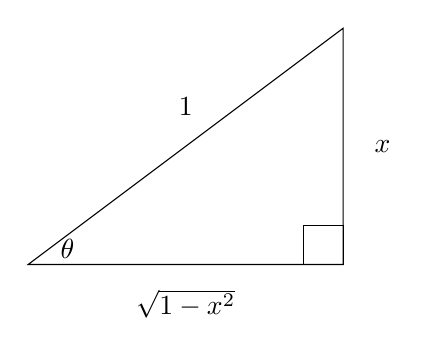
\begin{tikzpicture}
    \draw 
        (0,0)
        -- (4,0) 
        -- (4,3) 
        -- cycle;
    \draw 
        (0.5,0.2) node {$\theta$};
    \draw 
        (4.5, 1.5) node {$x$};
    \draw
        (2, -0.5) node {$\sqrt{1-x^2}$};
    \draw
        (2, 2) node {1};

    \draw (3.5, 0.5) rectangle (4, 0);
\end{tikzpicture}
Second case:
$$
\int{\frac{1}{\sqrt{a^2-x^2}}dx}=\int{\frac{1}{\sqrt{a^2(1-\frac{x^2}{a^2})}}dx}=\frac{1}{a}\int{\frac{1}{\sqrt{1-(\frac{x}{a})^2}}dx}
$$
$$
u=\frac{x}{a} ; du=\frac{1}{a}dx \Longrightarrow adu=dx
$$
$$
\frac{1}{a}\int{a\frac{1}{1-u^2}du}=\arcsin(u)+C=\arcsin(\frac{x}{a})+C
$$

\subsubsection{$\arctan(x)$}

$$
\int{\frac{1}{1+x^2}dx}=\arctan(x)+C
$$

$$
\frac{d}{dx}[y]=\frac{d}{dx}[\arctan(x)] \Longrightarrow \frac{d}{dx}[\tan(y)]=\frac{d}{dx}[x] \Longrightarrow \sec^2y*\frac{dy}{dx}=1 \Longrightarrow \frac{dy}{dx}=\cos^2y
$$
$$
\frac{dy}{dx}=\cos^2(\arctan(x))=\cos^2(\theta)=(\frac{1}{\sqrt{1+x^2}})^2=\frac{1}{1+x^2}
$$

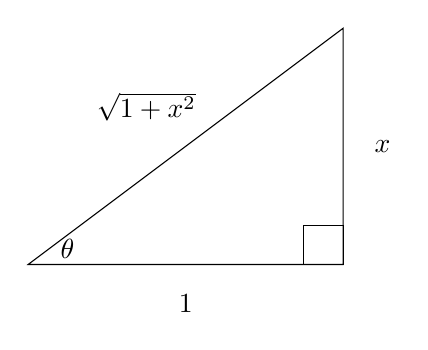
\begin{tikzpicture}
    \draw 
        (0,0)
        -- (4,0) 
        -- (4,3) 
        -- cycle;
    \draw 
        (0.5,0.2) node {$\theta$};
    \draw 
        (4.5, 1.5) node {$x$};
    \draw
        (2, -0.5) node {1};
    \draw
        (1.5, 2) node {$\sqrt{1+x^2}$};

    \draw (3.5, 0.5) rectangle (4, 0);
\end{tikzpicture} 
Second case:
$$
\int{\frac{1}{a^2+x^2}dx}=\int{\frac{1}{a^2(1+(\frac{x}{a})^2)}dx}=
\frac{1}{a}\int{\frac{1}{1+(\frac{x}{a})^2}dx}
$$
$$
u=\frac{x}{a} ; du=\frac{1}{a}dx \Longrightarrow adu=dx
$$
$$
\frac{1}{a}\int{\frac{1}{1+u^2}adu}=\arctan(u)+C=\arctan(\frac{x}{a})+C
$$


\subsubsection{$arcsec(x)$}
$$
\int{\frac{1}{x\sqrt{x^2-1}}dx}=arcsec(|x|)+C
$$

$$
\frac{d}{dx}[y]=\frac{d}{dx}[arcsec(|x|)] \Longrightarrow \frac{d}{dx}[\sec(y)]=\frac{d}{dx}[x] \Longrightarrow \sec(x)\tan(x)*\frac{dy}{dx}=1 
$$
$$
\frac{dy}{dx}=\frac{1}{\sec{x}\tan{x}}=\frac{1}{x\sqrt{x^2-1}}
$$

\begin{tikzpicture}
    \draw 
        (0,0)
        -- (4,0) 
        -- (4,3) 
        -- cycle;
    \draw 
        (0.5,0.2) node {$\theta$};
    \draw 
        (5, 1.5) node {$\sqrt{x^2-1}$};
    \draw
        (2, -0.5) node {1};
    \draw
        (1.5, 2) node {$x$};

    \draw (3.5, 0.5) rectangle (4, 0);
\end{tikzpicture}
Second case:
$$
\int{\frac{1}{x\sqrt{x^2-a^2}}dx}=
\int{\frac{1}{ax\sqrt{(\frac{x}{a})^2-1}}dx}
$$
$$
u=\frac{x}{a} ; du=\frac{1}{a}dx \Longrightarrow adu=dx
$$
$$
\frac{1}{a}\int{a\frac{1}{au\sqrt{u^2-1}}du}=\frac{1}{a}arcsec(|u|)+C=
\frac{1}{a}arcsec(|\frac{x}{a}|)+C
$$

The absolute value remains because of:
$$
\int{\frac{1}{|x|\sqrt{x^2-1}}dx}=arcsec(x)+C \Longrightarrow
\frac{|x|}{x}\int{\frac{1}{|x|\sqrt{x^2-1}}dx}=(arcsec(x)+C)\frac{|x|}{x} 
$$
$$
\Longrightarrow \int{\frac{1}{x\sqrt{x^2-1}}dx}=arcsec(|x|)+C
$$

\subsection{Esoteric $\sqrt{}$ Simplification}
The same methods can be used to simplify $\sqrt{}$ when \textbf{u-subsitution and all other methods have failed.}. Like the title suggests, these are esoteric at best.

\subsubsection{$\sqrt{a^2-x^2}$}

$$
x=a\sin(\theta); dx=a\cos(\theta)d\theta
$$
$$
\sqrt{a^2-x^2}=\sqrt{a^2-a^2\sin^2(\theta)}=\sqrt{a^2\cos^2(\theta)}=a\cos(\theta)
$$

\subsubsection{$\sqrt{a^2+x^2}$}

$$
x=a\tan(\theta); dx=a\sec^2(\theta)d\theta
$$
$$
\sqrt{a^2+x^2}=\sqrt{a^2+a^2\tan(\theta)}=\sqrt{a^2\sec^2(\theta)}=a\sec(\theta)
$$

\subsubsection{$\sqrt{x^2-a^2}$}
$$
x=a\sec(\theta); dx=a\sec(\theta)\tan(\theta)d\theta
$$
$$
\sqrt{x^2-a^2}=\sqrt{a^2\sec^2(\theta)-a^2}=\sqrt{a^2\tan^2(\theta)}=atan(\theta)
$$



\subsection{Completing the Square}
Completing the square can facilitate usage of the methods outlined above. An example would best illustrate this point:
$$
\int{\sqrt{5-4x-x^2}dx}=\int{\sqrt{5+4-(x^2+4x+4)}dx}=\int{\sqrt{9-(x+2)^2}dx}
$$
Since $\frac{d}{dx}[x+2]=1$, we can use the second-case derivative of $\arctan(x)$
$$
=\arctan(\frac{x+2}{3})+C
$$

\section{Trig Identity Integrals}
\subsection{Self Explanatory}
$$
\int{\cos(x)dx}=\sin(x) + C
$$
$$
\int{\sin(x)dx}=-\cos(x) + C
$$

\subsection{$\int{sec^2(x)dx}=tan(x) + C$}

We can derive it using Quotient Rule:
$$
\frac{d}{dx}[tan(x)]=\frac{d}{dx}[\frac{\sin(x)}{\cos(x)}]
$$
$$
\frac{d}{dx}[\frac{\sin(x)}{\cos(x)}]=\frac{\cos(x)*\frac{d}{dx}[\sin(x)]-\sin(x)*\frac{d}{dx}[\cos(x)]}{\cos^2(x)}
$$
$$
\frac{\cos(x)*\frac{d}{dx}[\sin(x)]-\sin(x)*\frac{d}{dx}[\cos(x)]}{\cos^2(x)}=\frac{\cos^2(x)-(-\sin^2(x))}{\cos^2(x)}
$$
Use the trig identity $\cos^2(x)+\sin^2(x)=1$:
$$
\frac{\cos^2(x)-(-\sin^2(x))}{\cos^2(x)}=\frac{1}{\cos^2(x)}=sec^2(x)
$$

\subsection{$\int{-csc^2(x)dx}=cot(x) + C$}

We can also derive it using Quotient Rule:
$$
\frac{d}{dx}[cot(x)]=\frac{d}{dx}[\frac{\cos(x)}{\sin(x)}]
$$
$$
\frac{d}{dx}[\frac{\cos(x)}{\sin(x)}]=\frac{\sin(x)*\frac{d}{dx}[\cos(x)]-\cos(x)*\frac{d}{dx}[\sin(x)]}{\sin^2(x)}
$$
$$
\frac{\sin(x)*\frac{d}{dx}[\cos(x)]-\cos(x)*\frac{d}{dx}[\sin(x)]}{\sin^2(x)} =\frac{-\cos^2(x)-\sin^2(x)}{\sin^2(x)}
$$
Use the trig identity $\cos^2(x)+\sin^2(x)=1$:
$$
\frac{-\cos^2(x)-\sin^2(x)}{\cos^2(x)}=\frac{-1}{\sin^2(x)}=-csc^2(x)
$$

\subsection{$\int{\sec(x)tan(x)dx}=\sec(x) + C$}
OR
$$
\int{\frac{\sin(x)}{\cos^2(x)}dx}=\sec(x) + C
$$
There are two methods to arrive at the following. One is to use u-subsitution and the other is to use the power rule and chain. Let's start with the easier one.

$$
\frac{d}{dx}[\sec(x) + C]=\frac{d}{dx}[\frac{1}{\cos(x)}+C]=\frac{d}{dx}[(\cos(x))^{-1}]=-(\cos(x))^{-2}*\frac{d}{dx}[\cos(x)]
$$
$$
-\frac{-\sin(x)}{\cos^2(x)}=\frac{\sin(x)}{\cos^2{x}}=\sec(x)tan(x)
$$

We can also just directly undo the chain rule.

$$
\int{\frac{\sin(x)}{\cos^2(x)}dx} 
$$
$$
u=\cos(x)
$$
$$
du=-\sin(x)dx
$$
$$
-\frac{du}{\sin(x)}=dx
$$
$$
\int{\frac{\sin(x)}{u^2}*-\frac{du}{\sin(x)}dx}=-\int{\frac{du}{u^2}}=u^{-1}+C=\sec(x)+C
$$

\subsection{$\int{csc(x)cot(x)dx}=\int{\frac{\cos(x)}{\sin^2(x)}dx}=-csc(x)+C$}

$$
\frac{d}{dx}[-csc(x)]=-\frac{d}{dx}[-\frac{1}{\sin(x)}]=\frac{1}{\sin^2(x)}*\frac{d}{dx}[\sin(x)]=\frac{\cos(x)}{\sin^2(x)}
$$

$$
u=\sin(x)\;du=\cos(x)dx\;\frac{du}{\cos(x)}=dx
$$
$$
\int{\frac{\cos(x)}{u^2}*\frac{du}{\cos(x)}}=-u^1+C=-csc(x)+C
$$

\subsection{$\int{tan(x)dx}=\ln|\sec(x)| + C$}
Let's break it into components and use u-subsitution:

$$
\int{tan(x)dx}=\int{\frac{\sin(x)}{\cos(x)}dx}
$$

Let's set u to be $\cos(x)$
$$
u=\cos(x)
$$
$$
du=-\sin(x)dx 
$$
$$
\frac{du}{-\sin(x)}=dx
$$

Now we have:
$$
\int{\frac{\sin(x)}{\cos(x)}dx}=\int{\frac{\sin(x)}{u}*\frac{du}{-\sin(x)}}
$$
$$
-\int{\frac{du}{u}}=-[\ln|u| + C]
$$
$$
-\ln|\cos(x)|+C_2
$$
\subsection{Again for $\int{cot(x)dx}$}

$$
\int{\frac{\cos(x)}{\sin(x)}dx}
$$
If we use u subsitution on the denominator:
$$
u=\sin(x)
$$
$$
du=\cos(x)dx
$$
$$
\frac{du}{cox(x)}=dx
$$
Sub it back in:
$$
\int{\frac{\cos(x)}{u}*\frac{du}{\cos(x)}}=\int{\frac{du}{u}}=\ln|u|+C=\ln|\sin(x)|+C
$$

\subsection{Algebraic:  $\int{\sec(x)dx}=\ln|\sec(x) + tan(x)| + C$} 
If you multiply this expression by a certain term, you will get an expression in the form $\int{\frac{du}{u}}$. Can you guess what it is?
$$
\int{\sec(x)dx}=\int{\sec(x)\frac{\sec(x)+tan(x)}{\sec(x)+tan(x)}dx}=\int{\frac{sec^2(x)+\sec(x)tan(x)}{\sec(x)+tan(x)}dx}
$$
using $u=\sec(x)+tan(x)$ and $du=sec^2(x)+\sec(x)tan(x)dx$
$$
\int{\frac{du}{u}}=\ln|u|+C=\ln|\sec(x)+tan(x)|+C
$$

\subsection{Similarly, $\int{csc(x)dx}=-\ln|csc(x) + cot(x)| + C$}
$$
\int{csc(x)dx}=\int{csc(x)\frac{csc(x)+cot(x)}{csc(x)+cot(x)}dx}=\int{\frac{-csc^2(x)-csc(x)cot(x)}{csc(x)+cot(x)}dx}
$$
using $u=csc(x)+cot(x)$ and $du=-csc^2(x)-csc(x)cot(x)dx$
$$
-\int{\frac{du}{u}}=-\ln|u|+C=-\ln|csc(x)+cot(x)|+C
$$
\subsection{$\int{\sin^2(x)dx}=\frac{1}{2}x-\frac{\sin(2x)}{4}+C$}
For this one, you need to rewrite $\sin^2(x)$ in a more easily integratable format. Recall that $\cos(2x)=\cos^2(x)-\sin^2(x)$, or $\cos(2x)=1-2\sin^2(x)$. Simplify a bit further and you get $\sin^2(x)=\frac{1-\cos(2x)}{2}$.
$$
\int{\frac{1-\cos(2x)}{2}dx}=\int{\frac{1}{2}dx}-\int{\frac{\cos(2x)}{2}dx}
$$
$$
u=2x\;du=2dx\; \frac{du}{2}=dx
$$
$$
\int{\frac{1}{2}dx}-\int{\frac{\cos(2x)}{2}dx}=\frac{1}{2}x-\frac{1}{2}\int{\frac{\cos(u)}{2}dx}+C=\frac{1}{2}x-\frac{\sin(u)}{4}+C=\frac{1}{2}x-\frac{\sin(2x)}{4}+C
$$
\subsection{$\int{\cos^2(x)dx}=\frac{1}{2}x+\frac{\sin(2x)}{4}+C$}
$$
\cos(2x)=\cos^2(x)-\sin^2(x)\; \cos(2x)=\cos^2(x)-(1-\cos^2(x))\; \cos(2x)=2\cos^2(x)-1
$$
$$
\cos^2(x)=\frac{\cos(2x)+1}{2}\; \int{\cos^2(x)dx}=\int{\frac{1}{2}dx}+\int{\frac{\cos(2x)}{2}dx}
$$
using the same u-sub logic:
$$
u=2x\; du=2dx\; \frac{du}{2}=dx
$$
$$
\frac{1}{2}x+\frac{1}{4}\int{\sin(u)du}+C=\frac{1}{2}x+\frac{\sin(2x)}{4}+C
$$
\section{Polynomials}
These problems assume a polynomial in the form:
$$
\int{\frac{A_1x^n+A_2x^{n-1}+...+A_n}{B_1x^m+B_2x^{m-1}+...+B_n}dx}
$$
Where $\{n,m\} \in \mathbb{R}$, $\{A_1, A_2, ... A_n\} \in \mathbb{R}$, $\{B_1, B_2, ... B_n\} \in \mathbb{R}$

\subsection{Long Division}

Where $n \geq m$, simply use long division.

\subsection{Partial Fraction Decomposition}
Where $n-1=m$ \\
Used to simplify:
$$
\int{\frac{A_1x+A_2}{B_1x^2+B_2x+B_3}dx}
$$
Best illustrated with an example:
$$
\int{\frac{-3x-7}{x^2-5x+6}dx}=\int{\frac{-3x-7}{(x-2)(x-3)}dx}
$$
We need to find an $A$ and $B$ such that:
$$
\frac{A}{x-2}*\frac{B}{x-3}=\frac{-3x-7}{(x-2)(x-3)}
$$
$$
\frac{A(x-3)}{(x-2)(x-3)}+\frac{B(x-2)}{(x-2)(x-3)}=\frac{-3x-7}{(x-2)(x-3)} \Longrightarrow A(x-3)+B(x-2)=-3x-7
$$
We can obtain the two following equations:
$$
Ax+Bx=-3x \Longrightarrow A+B=-3 \Longrightarrow B=-3-A
$$
$$
-3A-2B=-7
$$
Subsitute:
$$
-3A-2(-3-A)=-7 \Longrightarrow -3A+6+2A=-7 \Longrightarrow -A=-13 \Longrightarrow A=13
$$
$$
B=-3-A \Longrightarrow B=-3-13 \Longrightarrow B=-16
$$

Now we can integrate the two sections individually:
$$
\int{\frac{-3x-7}{(x-2)(x-3)}dx}=13\int{\frac{1}{x-2}dx}-16\int{\frac{1}{x-3}dx}=13\ln|x-2|-16\ln|x-3|+C
$$
\section{Improper Integrals}
$$
\int^\infty_a{f(x)dx}=\lim_{b \to \infty}{\int^b_a{f(x)dx}}
$$

Similarly:
$$
\int^\infty_{-\infty}{f(x)dx}=\int^\infty_a{f(x)dx}+\int^a_{-\infty}{f(x)dx}=
\lim_{b \to \infty}{\int^b_a{f(x)dx}}+\lim_{c \to -\infty}{\int^a_c{f(x)dx}}
$$

The integral may not always exist. For polynomials,

$$
\lim_{x \to \infty}{\frac{x^n...}{x^m...}} \in \mathbb{R} 
\iff 
m\geq n + 2
$$

If the degree of the denominator is two higher than the numerator, then the integral will exist.
\section{Riemann Sum}
A typical Riemann Sum will equal the general expression:
$$
\sum{f(x_i)\Delta x}
$$

\subsection{Left Riemann Sum}

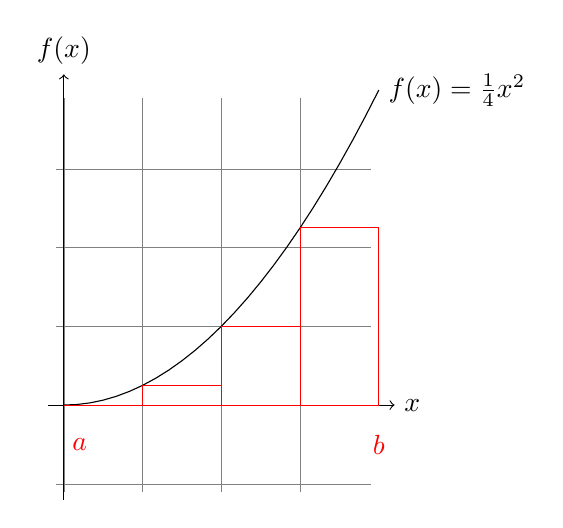
\begin{tikzpicture}[domain=0:4]
    \draw[very thin,color=gray] (-0.1,-1.1) grid (3.9,3.9);
    \draw[->] (-0.2,0) -- (4.2,0) node[right] {$x$};
    \draw[->] (0,-1.2) -- (0,4.2) node[above] {$f(x)$};
    \draw plot (\x,0.25*\x^2) node[right] {$f(x) =\frac{1}{4}x^2$};
    \draw[color=red] (0,0) rectangle (1,0);
    \draw[color=red] (1,0) rectangle (2,0.25);
    \draw[color=red] (2,0) rectangle (3,1);
    \draw[color=red] (3,0) rectangle (4,2.25);
    \draw[color=red] (0.2,-0.5) node {$a$};
    \draw[color=red] (4,-0.5) node {$b$};
\end{tikzpicture}

Let total steps be represented by $n$.
Let $i$ represent the current step
$$
\Delta x = \frac{b-a}{n}
$$
$$
f(x_i) = \frac{f(a+i\Delta x)}{n}
$$
Put them together:
$$
\sum_{i=0}^{n-1}{f(x_i)\Delta x} \Longrightarrow 
\sum_{i=0}^{n-1}{\frac{f(a+i\Delta x)}{n}\Delta x} \Longrightarrow
\sum_{i=0}^{n-1}{\frac{f(a+i\frac{b-a}{n}x)(b-a)}{n^2}}
$$

\subsection{Right Riemann Sum}
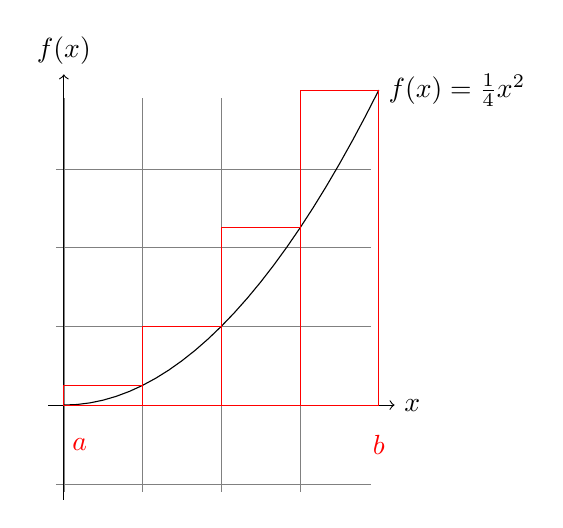
\begin{tikzpicture}[domain=0:4]
    \draw[very thin,color=gray] (-0.1,-1.1) grid (3.9,3.9);
    \draw[->] (-0.2,0) -- (4.2,0) node[right] {$x$};
    \draw[->] (0,-1.2) -- (0,4.2) node[above] {$f(x)$};
    \draw plot (\x,0.25*\x^2) node[right] {$f(x) =\frac{1}{4}x^2$};
    \draw[color=red] (0,0) rectangle (1,0.25);
    \draw[color=red] (1,0) rectangle (2,1);
    \draw[color=red] (2,0) rectangle (3,2.25);
    \draw[color=red] (3,0) rectangle (4,4);
    \draw[color=red] (0.2,-0.5) node {$a$};
    \draw[color=red] (4,-0.5) node {$b$};
\end{tikzpicture}

Nothing changes, except for the $\sum$ bounds:
$$
\sum_{i=1}^{n}{f(x_i)\Delta x} \Longrightarrow 
\sum_{i=1}^{n}{\frac{f(a+i\Delta x)}{n}\Delta x} \Longrightarrow
\sum_{i=1}^{n}{\frac{f(a+i\frac{b-a}{n}x)(b-a)}{n^2}}
$$

\subsection{Midpoint Riemann Sum}
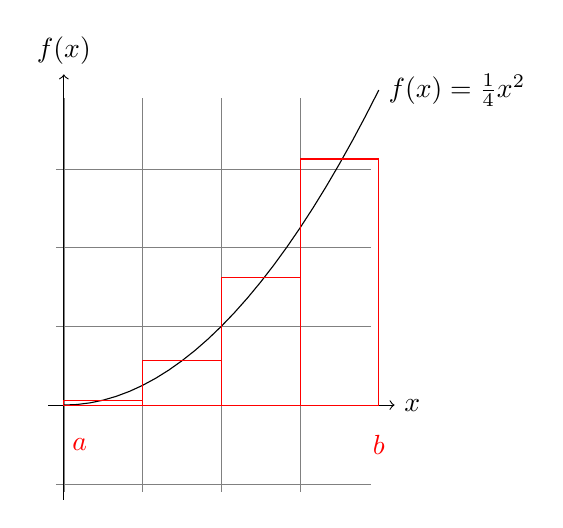
\begin{tikzpicture}[domain=0:4]
    \draw[very thin,color=gray] (-0.1,-1.1) grid (3.9,3.9);
    \draw[->] (-0.2,0) -- (4.2,0) node[right] {$x$};
    \draw[->] (0,-1.2) -- (0,4.2) node[above] {$f(x)$};
    \draw plot (\x,0.25*\x^2) node[right] {$f(x) =\frac{1}{4}x^2$};
    \draw[color=red] (0,0) rectangle (1,0.0625);
    \draw[color=red] (1,0) rectangle (2,0.5625);
    \draw[color=red] (2,0) rectangle (3,1.625);
    \draw[color=red] (3,0) rectangle (4,3.125);
    \draw[color=red] (0.2,-0.5) node {$a$};
    \draw[color=red] (4,-0.5) node {$b$};
\end{tikzpicture}

As the name suggests, you take the average of $f(x_i)$ and $f(x_{i+1})$. Instead of using $f(x_i)$, use $f(\frac{x_i+x_{i+1}}{2})$

$$
\sum_{i=0}^{n-1}{f(\frac{x_i+x_{i+1}}{2})\Delta x} \Longrightarrow 
\sum_{i=0}^{n-1}{\frac{f(\frac{a+i\Delta x + a + (i + 1)\Delta x}{2})}{n}\Delta x}=
\sum_{i=0}^{n-1}{\frac{f(\frac{2a+(2i+1)\Delta x}{2})}{n}\Delta x}
$$
$$
\Longrightarrow 
\sum_{i=0}^{n-1}{\frac{f(\frac{2a+(2i+1)\frac{b-a}{n}x}{2})(b-a)}{n^2}}
$$

\subsection{Trapezoidal Riemann Sum}
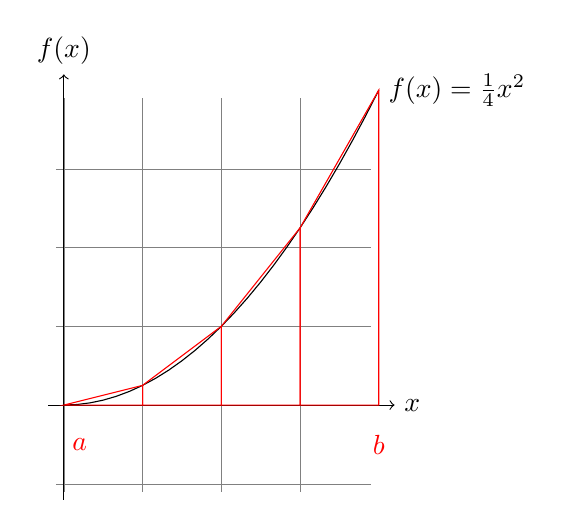
\begin{tikzpicture}[domain=0:4]
    \draw[very thin,color=gray] (-0.1,-1.1) grid (3.9,3.9);
    \draw[->] (-0.2,0) -- (4.2,0) node[right] {$x$};
    \draw[->] (0,-1.2) -- (0,4.2) node[above] {$f(x)$};
    \draw plot (\x,0.25*\x^2) node[right] {$f(x) =\frac{1}{4}x^2$};
    \draw[color=red] (0,0) -- (1,0.25) -- (1,0) -- cycle;
    \draw[color=red] (1,0) -- (1,0.25) -- (2,1) -- (2,0) -- cycle;
    \draw[color=red] (2,0) -- (2,1) -- (3,2.25) -- (3,0) -- cycle;
    \draw[color=red] (3,0) -- (3,2.25) -- (4,4) -- (4,0) -- cycle;
    \draw[color=red] (0.2,-0.5) node {$a$};
    \draw[color=red] (4,-0.5) node {$b$};
\end{tikzpicture}

Take the average of the two y-values instead. Instead of using $f(x_i)$, use $\frac{f(x_i)+f(x_{i+1})}2$
$$
\sum_{i=0}^{n-1}{\frac{f(x_i)+f(x_{i+1})}2\Delta x} \Longrightarrow 
\sum_{i=0}^{n-1}{\frac{f(a+i\Delta x)+f(a+(i+1)\Delta x)}{2n}\Delta x} 
$$
$$
\Longrightarrow
\sum_{i=0}^{n-1}{\frac{(f(a+i\frac{b-a}{n}x)+f(a+(i+1)\frac{b-a}{n}x)(b-a)}{2n^2}}
$$

\section{Distance}

The distance of the curve is represented by the following:

\begin{align*}
    \text{arc length}=\sqrt{(\Delta x)^2+(\Delta y)^2}=\sqrt{1+\left(\frac{\Delta y}{\Delta x}\right)^2}\Delta x \\
    \Longrightarrow \int{\sqrt{1+(\frac{dy}{dx})^2}}dx
\end{align*}

\subsection{Example}

These problems are taken from \textit{Calculus for the AP Course} by Michael Sullivan. 

\begin{enumerate}
    \item Let $g$ be the function defined by $g(x)=\int_1^x{\sqrt{9t^2-1}}dt$. Which integral represents the graph of $g$ on the interval $[2,5]$?

    Let $f(x)=\sqrt{9t^2-1}$. Let $F(x)$ represent its antiderivative. 

    \begin{align*}
        g(x)=F(x)-F(1) \\
        g'(x)=\sqrt{9x^2-1} \\
        \int_2^5{\sqrt{1+9x^2-1}dx}=\int_2^5{3x}dx
    \end{align*}
\end{enumerate}

\end{document}
